\chapter{On logical correspondence}
\label{chapter-correspondence}

In Part 1, we defined \sls, a logical framework of substructural
logical specifications. For the purposes of this thesis, we are
primarily interested in using \sls~as a framework for specifying the
operational semantics of programming languages, especially stateful
and concurrent programming languages. This is not a new idea: one of
the original case studies on CLF specification described the semantics
of Concurrent ML \cite{cervesato02concurrent} in a specification style
termed {\it substructural operational semantics}, or SSOS, by Pfenning
\cite{pfenning04substructural}. 

The design space of substructural operational semantics is extremely
rich, and many styles of SSOS specification have been proposed
previously. It is therefore helpful to have design principles that
allow us to both {\it classify} different styles of presentation and
{\it predict} what style(s) we should adopt based on what our goals
are. In this chapter, I propose a classification scheme for
substructural operational semantics based on three major specification
styles.  Each of these styles is more expressive than the last.

\begin{itemize}
\item The {\it natural semantics}, or big-step operational semantics,
  is an existing and well-known specification style (and not a
  substructural operational semantics). It is convenient for the
  specification of pure programming languages.

\item The {\it ordered abstract machine semantics} is a generalization
  of abstract machine semantics that can be naturally specified in
  \sls; this specification style naturally handles stateful and
  parallel programming language features
  \cite{pfenning09substructural}.

\item The {\it destination-passing semantics} is the style of
  substructural operational semantics first explored in CLF by
  Cervesato et al.~\cite{cervesato02concurrent}. It allows for the
  natural specification of features that incorporate 
  communication and non-local transfer of control. Destination-passing
  semantics are classified into two subspecies: those with linear
  continuations and those with persistent continuations. Persistent
  continuations are necessary to give a substructural operational
  semantics to languages with first-class continuations.
\end{itemize}


\begin{figure}
\begin{center}
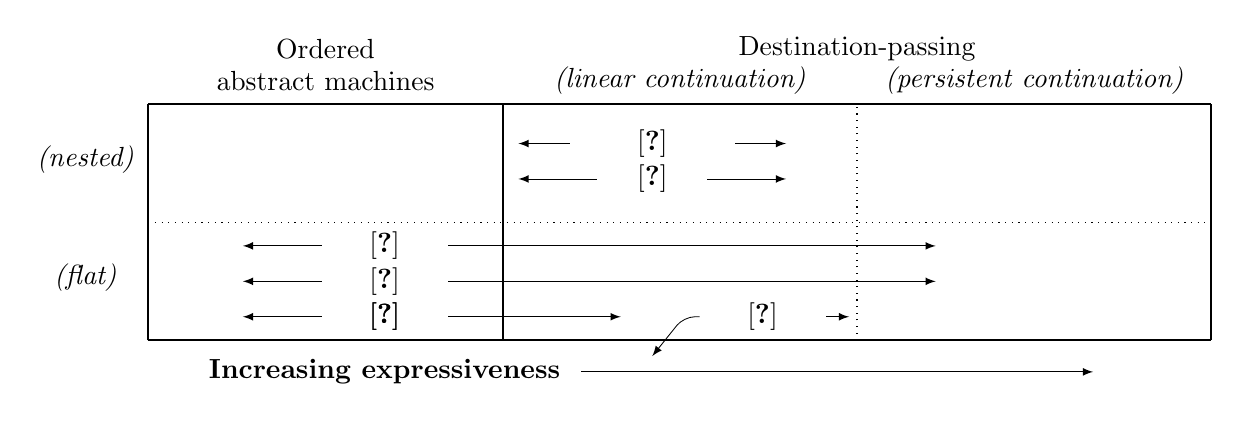
\begin{tikzpicture} 
\draw[thick](0cm,0cm) -- (0cm,3cm);
\draw (2.25,3.7) node{Ordered};
\draw (2.25,3.3) node{abstract machines};
%
\draw[thick](4.5cm,0cm) -- (4.5cm,3cm);
\draw (9,3.7) node{Destination-passing};
\draw (6.75,3.3) node{\it (linear continuation)};
%
\draw[dotted](9cm,0cm) -- (9cm,3cm);
\draw (11.25,3.3) node{\it (persistent continuation)};
%
\draw[thick](13.5cm,0cm) -- (13.5cm,3cm);
%
\draw[thick](0,0) -- (13.5,0);
\draw[dotted] (0,1.5) -- (13.5,1.5);
\draw[thick](0,3) -- (13.5,3);
%
\draw (-.8,2.3) node{\it (nested)};
%
\draw (-.8,0.8) node{\it (flat)};
%
\draw (3,1.2) node{\cite{pfenning04substructural}};
\draw (3,.75) node{\cite{pfenning09substructural}};
\draw (3,.3) node{\cite{simmons11logical}};
\draw (3,.3) node{\cite{simmons11logical}};
\draw (7.8,.3) node{\cite{pfenning12substructural}};
\draw (6.4,2.5) node{\cite{cervesato02concurrent}};
\draw (6.4,2.05) node{\cite{schacknielsen07induction}};
\draw (3,-.4) node{\bf Increasing expressiveness};
%
\pgfsetarrowsstart{latex} 
\pgfsetlinewidth{.3pt} 
\pgfusepath{stroke} 
\draw (1.2,1.2) -- (2.2,1.2);
\draw (10,1.2) -- (3.8,1.2);
\draw (1.2,.75) -- (2.2,.75);
\draw (10,.75) -- (3.8,.75);
\draw (1.2,.3) -- (2.2,.3);
\draw (6,.3) -- (3.8,.3);
\draw[rounded corners=4pt] (6.4,-.2) -- (6.8,.3) -- (7,.3);
\draw (8.9,.3) -- (8.6,.3);
\draw (4.7,2.5) -- (5.35,2.5);
\draw (4.7,2.05) -- (5.7,2.05);
\draw (8.1,2.5) -- (7.45,2.5);
\draw (8.1,2.05) -- (7.1,2.05);
%
\draw (12,-.4) -- (5.5,-.4);
\end{tikzpicture} 
\end{center}
\caption{Classification of existing work on SSOS specifications.}
\label{fig:class-prevwork}
\end{figure}

This classification of substructural operational semantics is
illustrated graphically in Figure~\ref{fig:class-prevwork}. Existing
published work on substructural operational semantics specifications
is placed in the figure, with arrows indicating the range of styles
that are considered in the cited work.  With the possible exception of
certain aspects of the SSOS presentation in Pfenning's course notes
\cite{pfenning12substructural}, the taxonomy described above captures
the scope of previous work.

The statement that each specification style is strictly more
expressive than the last is formal: there are automatic and
provably-correct transformations from the less expressive styles
(natural semantics and ordered abstract machines) to the more
expressive styles (ordered abstract machines and destination-passing,
respectively).  Our investigation of provably-correct transformations
on \sls~specifications therefore justifies our classification scheme
for SSOS specifications. We call this idea the {\it logical
  correspondence}, and it is the focus of this part of the thesis:

\begin{quote} 
  {\bf Thesis (part II):} A logical framework based on a rewriting
  interpretation of substructural logic supports many styles of
  programming language specification. These styles can be formally
  classified and connected by considering general transformations on
  logical specifications.
 
  Generally applicable transformations on logical
  specifications are also useful for deriving manifestly correct
  program analyses from those operational semantics specifications.
\end{quote} 

\noindent
In this introductory chapter, we will outline our use of logical
correspondence and connect it to previous work. The development of the
logical correspondence as presented in this chapter, as well as the
operationalization and defunctionalization transformations presented
in the next chapter, represent joint work with Ian Zerny.

\section{Logical correspondence}

As stated above, we will primarily discuss and connect three different
styles that are used for specifying the semantics of programming
languages. Natural semantics is a high-level, declarative style of
specification inspired by Plotkin's structural operational semantics
(SOS) \cite{plotkin04structural,kahn87natural}. While Kahn et
al.~defined the term broadly, natural semantics has been consistently
connected with the big-step operational semantics style discussed in
the introduction, where the judgment $e \Downarrow v$ expresses that
the $e$ evaluates to the value $v$:
\[
\infer[{\sf ev/lam}]
{\lambda x. e \Downarrow \lambda x. e \mathstrut}
{}
\quad
\infer[{\sf ev/app}]
{e_1\,e_2 \Downarrow v \mathstrut}
{e_1 \Downarrow \lambda x.e
 &
 e_2 \Downarrow v_2
 &
 [v_2/x]e \Downarrow v \mathstrut}
\]
% Plotkin's SOS, in contrast, has been consistently identified with a
% small-step operational semantics style in which a judgment $e \mapsto
% e'$ expresses that the expression $e$ makes a single transition to the
% expression $e'$, and an auxilary judgment $e\,{\sf value}$ expresses
% that the expression $e$ is a value and not expected to make any
% further transitions. The usual SOS specification for call-by-value
% evaluation of the lambda calculus looks like this:
% \[
% \infer%[{\sf value/lam}]
% {\lambda x.e\,{\sf value} \mathstrut}
% {}
% \quad
% \infer%[{\sf step/app1}]
% {e_1\,e_2 \mapsto e_1'\,e_2 \mathstrut}
% {e_1 \mapsto e_1' \mathstrut}
% \quad
% \infer%[{\sf step/app2}]
% {v_1\,e_2 \mapsto v_1\,e_2' \mathstrut}
% {v_1\,{\sf value}
%  &
%  e_2 \mapsto e_2' \mathstrut}
% \quad
% \infer%[{\sf step/appred}]
% {(\lambda x.e)\,v_2 \mapsto [v_2/x]e \mathstrut}
% {v_2\,{\sf value}}
% \]

Early work on natural semantics emphasized a dual interpretation of
specifications. The primary interpretation of natural semantics
specifications was {\it operational}: natural semantics were
implemented in the (non-logical) specification framework TYPOL that
compiled natural semantics specifications into executable Prolog
programs \cite{clement85natural}. It is also possible to natural
semantics specifications as inductive definitions; this interpretation
allows proofs to be performed by induction over the structure of a
natural semantics derivation \cite{clement86simple}.

The operational interpretation of natural semantics assigns a more
specific meaning to expressions than the inductive definition does.
For example, the rule ${\sf ev/app}$, the natural semantics does not
specify whether $e_1$ or $e_2$ should be evaluated in some particular
order or in parallel; the TYPOL-to-Prolog compiler could have
reasonably made several choices in such a situation. More critically,
interpreting the natural semantics as an inductive definition does not
allow us to distinguish non-termination (searching forever for a $v$
such that $e \Downarrow v$) from failure (concluding finitely that
there is no $v$ such that $e \Downarrow v$).

We will present a transformation from \sls-encoded natural semantics
specifications into ordered abstract machines by a transformation
called {\it operationalization}; operationalization is an
interpretation of natural semantics specifications that makes
evaluation order and parallelism explicit and that enables reasoning
about the difference between non-termination and failure. In turn,
ordered abstract machine specifications can be transformed into
destination-passing specifications by a transformation called {\it
  destination-adding}.  Destination-passing specifications can then be
transformed into a collecting semantics by {\it approximation}, which
lets us obtain program analyses like control flow analysis. These
major transformations are presented graphically in
Figure~\ref{fig:class-transform}.

\begin{figure}
\begin{center}
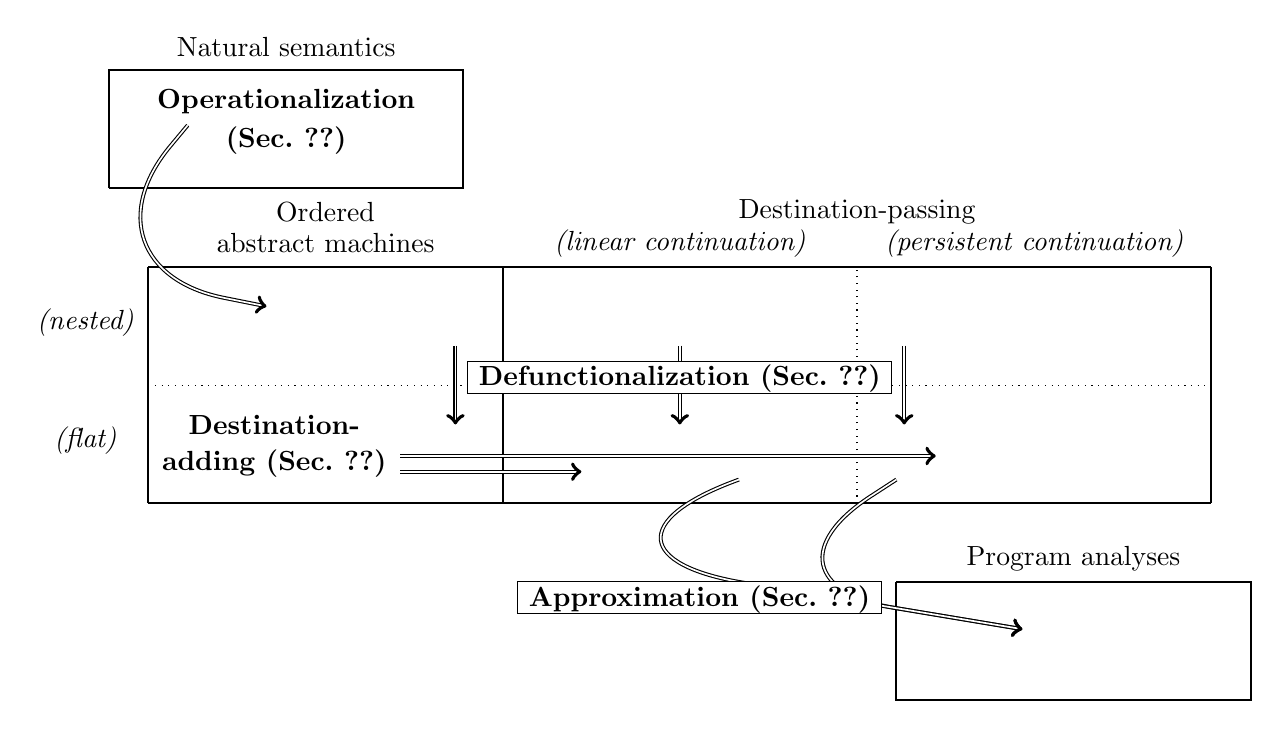
\begin{tikzpicture}
\draw (1.75,5.8) node{Natural semantics};
\draw[thick](-.5cm,4cm) -- (-.5cm,5.5cm) -- (4cm,5.5cm) 
  -- (4cm,4cm) -- (-.5cm,4cm);
%
\draw (11.75,-.7) node{Program analyses};
\draw[thick](9.5cm,-1cm) -- (9.5cm,-2.5cm) -- (14cm,-2.5cm) 
  -- (14cm,-1cm) -- (9.5cm,-1cm);
%
\draw[thick](0cm,0cm) -- (0cm,3cm);
\draw (2.25,3.7) node{Ordered};
\draw (2.25,3.3) node{abstract machines};
%
\draw[thick](4.5cm,0cm) -- (4.5cm,3cm);
\draw (9,3.7) node{Destination-passing};
\draw (6.75,3.3) node{\it (linear continuation)};
%
\draw[dotted](9cm,0cm) -- (9cm,3cm);
\draw (11.25,3.3) node{\it (persistent continuation)};
%
\draw[thick](13.5cm,0cm) -- (13.5cm,3cm);
%
\draw[thick](0,0) -- (13.5,0);
\draw[dotted] (0,1.5) -- (13.5,1.5);
\draw[thick](0,3) -- (13.5,3);
%
\draw (-.8,2.3) node{\it (nested)};
%
\draw (-.8,0.8) node{\it (flat)};
%
\draw[double,->] (3.9,2) -- (3.9,1);
\draw[double,->] (6.75,2) -- (6.75,1);
\draw[double,->] (9.6,2) -- (9.6,1);
\draw (6.75,1.6) node {\fboxsep=0pt\fbox{\colorbox{white}{\rule[-0.5ex]{0em}{2.5ex}\bf ~Defunctionalization~(Sec.~\ref{sec:defunctionalization})~}}};
%
\draw (1.75,5.1) node {\bf Operationalization};
\draw (1.75,4.6) node {\bf (Sec.~\ref{sec:operationalization})~};
\draw[double,->,rounded corners=2cm] (.5,4.8) -- (-1,3) -- (1.5,2.5);
%
\draw (1.6,1) node {\bf Destination-};
\draw (1.6,.5) node {\bf adding (Sec.~\ref{sec:destination-adding})};
\draw[double,->] (3.2,.6) -- (10,.6);
\draw[double,->] (3.2,.4) -- (5.5,.4);
%
\draw[double,->,rounded corners=2cm] (9.5,.3) -- (7.5,-1) -- (11.1,-1.6);
\draw[double,->,rounded corners=2.5cm] (7.5,.3) -- (5.1,-.6) -- (11.1,-1.6);
\draw (7,-1.2) node {\fboxsep=0pt\fbox{\colorbox{white}{\rule[-0.5ex]{0em}{2.5ex}\bf ~Approximation~(Sec.~\ref{sec:abstraction})~}}};
\end{tikzpicture} 
\end{center}
\caption{Major transformations on \sls~specifications.}
\label{fig:class-transform}
\end{figure}

There are many other smaller design decisions that can be made in the
creation of a substructural operational semantics. Only one is
graphically represented in
Figures~\ref{fig:class-prevwork}~and~\ref{fig:class-transform}, the
distinction between {\it nested} and {\it flat}
specifications. This distinction applies to all concurrent
\sls~specifications, not just those that specify substructural
operational semantics. Flat
specifications include rewriting rules $\left( p_1 \fuse \ldots \fuse
  p_n \lefti \{ q_1 \fuse \ldots \fuse q_m \} \right)$ where the head
of the rule $\{ q_1 \fuse \ldots \fuse q_m \}$ contains only atomic
propositions. Nested \sls~specifications, on the other hand,
contain {\it rules} in the conclusions of rules; when the rule fires,
the resulting process state contains the rule. An example is given 
in Figure~\ref{fig:ho-evo-ex}.
A rule $A^+ \lefti \{ B^+ \}$ in the context can only fire if a piece 
of the context
matching $A^+$ appears to its right, so  $\left(x{:}\susp{\sf p1(c)}, ~
y{:}\istrue{\left( {\sf p1(c)} \lefti \{ {\sf p2(c)} \} \right)}\right)
\leadsto \left(z{:}\susp{\sf p2(c)}\right)$, whereas 
$\left(y{:}\istrue{\left( {\sf p1(c)} \lefti \{ {\sf p2(c)} \} \right)},~
x{:}\susp{\sf p1(c)}\right)
\not \leadsto$. 
%
The choice of nested versus flat specification does not
impact expressiveness, but it does influence our ability to read
specifications (opinions differ as to which style is clearer) and 
the ways we reason about them.

\begin{figure}
\begin{align*}
x_1{:}\susp{{\sf p2}({\sf c})}, ~~
x_2{:}\susp{{\sf p1}({\sf c})}, ~~
x_3{:}\istrue{(\forall x.\,{\sf p_1}(x) 
                \lefti \{ {\sf p_2}(x) \lefti \{ {\sf p_3}(x) \} \})}, ~~
x_4{:}\istrue{({\sf p3}({\sf c}) \lefti \{ {\sf p_4} \})} & \\
\leadsto ~~~ 
x_1{:}\susp{{\sf p2}({\sf c})}, ~~
x_5{:}\istrue{({\sf p_2}({\sf c}) \lefti \{ {\sf p_3}({\sf c}) \})}, ~~
x_4{:}\istrue{({\sf p3}({\sf c}) \lefti \{ {\sf p_4} \})} & \\
\leadsto ~~~ 
x_6{:}\susp{{\sf p3}({\sf c})}, ~~
x_4{:}\istrue{({\sf p3}({\sf c}) \lefti \{ {\sf p_4} \})} & \\
\leadsto ~~~ 
x_7{:}\susp{{\sf p_4}} & 
\end{align*}
\caption{Evolution of a nested \sls~process state (${\sf p1}$, ${\sf
  p2}$ and ${\sf p3}$ are all ordered atomic propositions).}
\label{fig:ho-evo-ex}
\end{figure}

Other distinctions between \sls~specifications can be understood in
terms of nondeterministic choices that can be made by the various
transformations we consider. For example, the operationalization
transformation can produce ordered abstract machines that evaluate
subcomputations in parallel or in sequence, and the destination-adding
transformation can make continuations either linear or persistent. In
general, one source specification (a natural semantics or an ordered
abstract machine specification) can give rise to several different
target specifications (ordered abstract machine specifications or
destination-passing specifications). The correctness of the
transformation then acts as a simple proof of the equivalence of the
several target specifications.

The nondeterministic choices that transformations can make give us a
rigorous vocabulary for describing choices that otherwise seem
ad hoc. An example of this can be found in the paper that introduced
the destination-adding and approximation transformations
\cite{simmons11logical}. In that article, we had to motivate an ad-hoc
change to the usual abstract machine semantics. In this thesis, by the
time we encounter a similar specification in Chapter 8, we will be
able to see that this change corresponds to omitting tail-recursion
optimization in the process of operationalization.

\section{Related work}

This part of the thesis draws from many different sources of
inspiration. In this section, we survey this related work and, where
applicable, outline how our use of logical correspondence differs from
existing work.

\subsection*{Partiality in deductive computation}

The genesis of the operationalization transformation discussed in
Chapter~6 can be found in the treatment of the operational semantics
of LF in Tom Murphy VII's thesis~\cite{murphy08modal}; this treatment
can be seen as a synthesis of the operational interpretation of
natural semantics explored in Cl\'ement's et al.'s early work on
natural semantics in TYPOL work and the approach to theorem proving
pioneered by Twelf~\cite{pfenning99system}.

In his thesis, Murphy described a natural semantics for Lambda 5, a
distributed programming language, and encoded that specification in
Twelf. He then wanted to interpret that natural semantics as an {\it
  operational} semantics for Lambda 5 in the style of Cl\'ement et
al., which is a natural application of Twelf's logic program
interpretation \cite{michaylov91natural}.  However, Murphy also wanted
to prove a safety property for his language in Twelf, and the usual
approach to theorem proving in Twelf involves treating specifications
as inductive definitions. As discussed above, natural semantics do not
distinguish non-termination (which is safe) from failure (which
indicates underspecification and is therefore unsafe).

Theorem proving in Twelf involves interpreting proofs as logic
programs, and Murphy was able to use the checks Twelf performs on
proofs to describe a special purpose partiality directive. If a logic
program passed this special directive, Murphy could conclude that
moded proof search would never fail and never backtrack, though it
might diverge. This check amounted to a proof of safety (progress and
preservation) for the operational interpretation of his natural
semantics. I believe that every other existing proof of
safety\footnote{Progress in particular is the theorem of concern:
  proving preservation for a big-step operational semantics is
  straightforward.} for a big-step operational semantics is either
classical (like Leroy and Grall's approach, described below) or else
depends on a separate proof of equivalence with a small-step
operational semantics.

Murphy's proof only works because his formulation of Lambda 5 was {\it
  intrinsically typed}, meaning that, using the facilities provided by
LF's dependent types, he enforced that only well-typed terms could
possibly be evaluated. (His general proof technique should apply more
generally, but it would take much more work to express the check in
Twelf.)  The operationalization transformation is a way to
automatically derive a correct small-step semantics from the big-step
semantics by making the internal structure of a deductive computation
explicit as a concurrent computation. Having made this structure
accessible, we can explicitly represent complete, unfinished, and
stuck (or failing) computations as concurrent traces and reason about
these traces with a richer set of tools than the limited set Murphy
successfully utilized.

\subsection*{A coinductive interpretation}

Murphy proved safety for a natural semantics specification by
recovering the original operational interpretation of natural semantics
specifications as logic programs and using Twelf's facilities for
reasoning about logic programs.  Leroy and Grall, in
\cite{leroy09coinductive}, suggest a novel {\it coinductive}
interpretation of natural semantics specifications. Coevaluation $e
\Downarrow^{\sf co} v$ is defined as the {\it greatest} fixed point of
the following rules:
\[
\infer%[{\sf evco/lam}]
{\lambda x. e \Downarrow^{\sf co} \lambda x. e \mathstrut}
{}
\quad
\infer%[{\sf evco/app}]
{e_1\,e_2 \Downarrow^{\sf co} v \mathstrut}
{e_1 \Downarrow^{\sf co} \lambda x.e
 &
 e_2 \Downarrow^{\sf co} v_2
 &
 [v_2/x]e \Downarrow^{\sf co} v \mathstrut}
\]
Aside from the ${\sf co}$ annotation and the different interpretation,
these rules are syntactically identical to the natural semantics above
that were implicitly given an inductive interpretation.

Directly reinterpreting the inductive specification as a coinductive
specification doesn't quite produce the right result in the end. For
some diverging terms like $\omega = (\lambda x.\,x\,x)\,(\lambda
x.\,x\,x)$, we can derive $\omega \Downarrow^{\sf co} e$ for any
expression $e$, including expressions that are not values and
expressions with no relation to the original term. Conversely, there
are diverging terms ${\it Div}$ such that ${\it Div} \Downarrow^{\sf
  co} e$ is not derivable for {\it any} $e$.\footnote{Leroy and Grall
  discuss a counterexample due to Filinski: ${\it Div} = {\it Y}{\it
    F}x$, where $\it Y$ is the fixed-point combinator $\lambda
  f.\,(\lambda x.\,f\,(\lambda v.\,(x\,x)\,v))\,(\lambda
  x.\,f\,(\lambda v.\,(x\,x)\,v))$ and $\it F$ is $\lambda f.\,\lambda
  x.\,(\lambda g.\,\lambda y.\,g\,y)\,(f\,x)$
  \cite{leroy09coinductive}.} As a result, Leroy and Grall also give a
coinductive definition of diverging terms $e \Downarrow^\infty$ that
uses references inductively-defined evaluation judgment $e \Downarrow v$:
\[
\infer%[{\sf div/app1}]
{e_1\,e_2 \Downarrow^\infty}
{e_1 \Downarrow^\infty}
\quad
\infer%[{\sf div/app2}]
{e_1\,e_2 \Downarrow^\infty}
{e_1 \Downarrow v_1
 & 
 e_2 \Downarrow^\infty}
\quad
\infer%[{\sf div/app3}]
{e_1\,e_2 \Downarrow^\infty}
{e_1 \Downarrow \lambda x.\,e
 & 
 e_2 \Downarrow v_2
 &
 [v_2/x]e \Downarrow^\infty}
\]
Now diverging expressions are fully characterized as derivations for
which $e \Downarrow^\infty$ is derivable with an infinite derivation
tree. With this definition, Leroy and Grall prove a type safety
property: if $e$ has type $\tau$, then either $e \Downarrow v$ or $e
\Downarrow^{\infty}$.  However, the disjunctive character of this
theorem means that a constructive proof of type safety would be
required to take a typing derivation $e : \tau$ as input and produce
as output either a proof of termination $e \Downarrow v$ or a proof of
divergence $e \Downarrow^\infty$. This implies that a constructive
type safety theorem would need to decide termination, and so it is
unsurprising that type safety is proved classically by Leroy and
Grall.

We suggest that the operationalization transformation, seen as a
logical extension to Murphy's methodology, is superior to the
coinductive (re)interpretation as a way of understanding the behavior
of infinite terms in the natural semantics. Both approaches
reinterpret natural semantics in an operational way, but the
operationalization transformation gives us a satisfactory treatment of
diverging terms without requiring the definition of an additional
coinductive judgment $e \Downarrow^\infty$. And even {\it with} the
addition of the coinductively defined judgment $e \Downarrow^\infty$,
coinductive big-step operational semantics have significant issues
handling nondeterministic languages, a point that we will elaborate on
in Section~\ref{sec:absmachine-nondeterminism}.

\subsection*{The functional correspondence}

The ordered abstract machine that results from our operationalization
transformation corresponds to a standard abstract machine model (a
statement that is made precise
Section~\ref{sec:nat-ssos-adequacy}). In this sense, the logical
correspondence has a great deal in common with the {\it functional
  correspondence} of Ager, Danvy, Midtgaard, and
others~\cite{ager03functional,ager04functional,ager05functional,
  danvy08defunctionalized,danvy12interderiving}. 

The goal of the functional correspondence is to encode various styles
of semantic specifications (natural semantics, abstract machines,
small-step structural operational semantics, environment semantics,
etc.)~as functional programs. It is then possible to show that these
styles can be related by off-the-shelf and fully correct
transformations on functional programs. The largest essential
difference between the functional and logical correspondences, then,
is that the functional correspondence acts on functional programs,
whereas the logical correspondence acts on specifications encoded in a
logical framework (in our case, the logical framework \sls).

However, the functional correspondence as given assumes that semantic
specifications are adequately represented as functional programs. The
correspondence of the encoding an the ``on paper'' semantics is an
assumed prerequisite in work on the functional correspondence. In
contrast, by basing the logical correspondence upon the \sls~framework
we make it possible to reason formally and precisely about adequate
representation. The functional correspondence also shares some of the
coinductive reinterpretation's difficulties in dealing with
nondeterministic and parallel execution: it seems to be the case that
a nondeterministic or parallel functional language would be necessary
to faithfully encode nondeterministic or parallel programming language
features.

\subsection*{Transformation on specifications}

Two papers by Hannan and Miller \cite{hannan92operational} and Ager
\cite{ager04natural} are the most closely related to our work in this
portion of the thesis. Both papers propose operationalizing natural
semantics specifications as abstract machines by provably correct and
general transformations on logical specifications (in the case of
Hannan and Miller) or on specifications in the special-purpose
framework of L-attributed natural semantics (in the case of Ager).

A major difference in this case is that both lines of
work result in {\it deductive} specifications of abstract
machines. Our translation into concurrent specifications has the
advantage of exploiting parallelism, and also opens up specifications to
the modular inclusion of stateful and concurrent features, as we will
discuss in Section~\ref{sec:richer-ordered-abstract}.


\section{Transformation and modular extension}
\label{sec:the-point-is-modular-extension}

\begin{figure}
\begin{center}
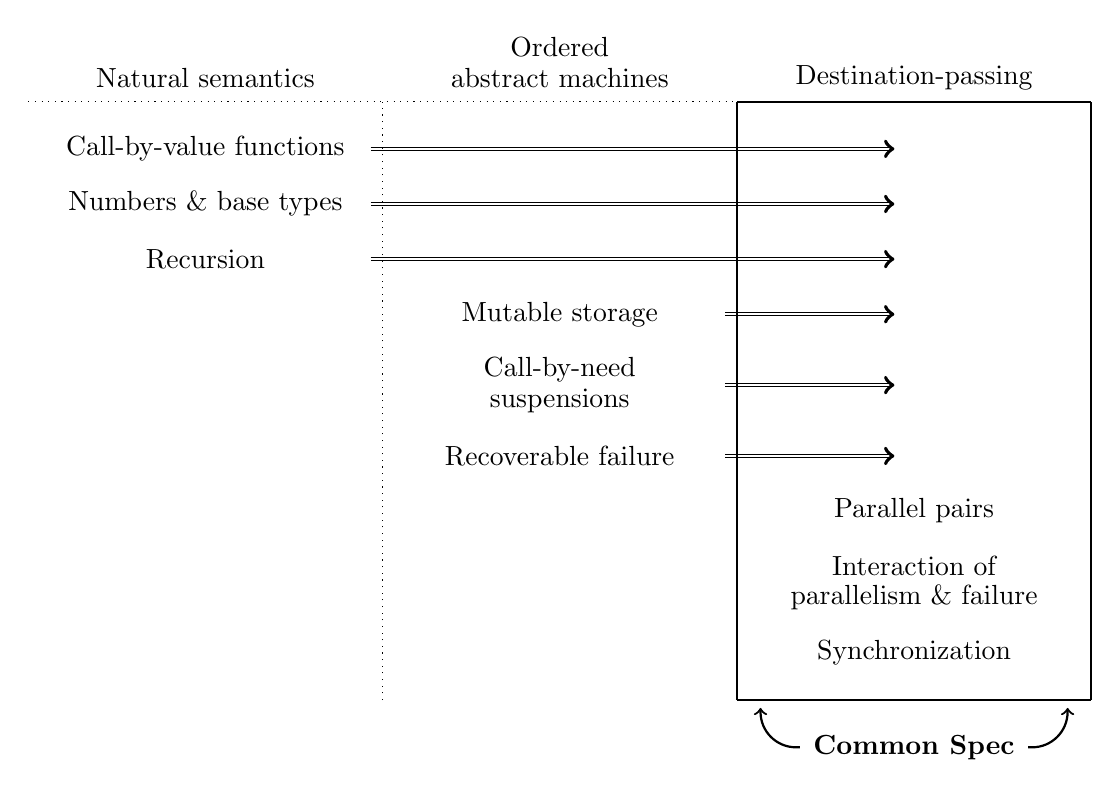
\begin{tikzpicture}
%\draw[thick](-4.5cm,0cm) -- (-4.5cm,3cm);
\draw (-2.25,3.3) node{Natural semantics};
%
\draw (-2.25,2.4) node{Call-by-value functions};
\draw[double,->] (-.15,2.4) -- (6.5,2.4);
\draw (-2.25,1.7) node{Numbers \& base types};
\draw[double,->] (-.15,1.7) -- (6.5,1.7);
\draw (-2.25,1) node{Recursion};
\draw[double,->] (-.15,1) -- (6.5,1);
%
\draw[dotted](0cm,-4.6cm) -- (0cm,3cm);
\draw (2.25,3.7) node{Ordered};
\draw (2.25,3.3) node{abstract machines};
%
\draw (2.25,.3) node{Mutable storage};
\draw[double,->] (4.35,.3) -- (6.5,.3);
\draw (2.25,-.4) node{Call-by-need};
\draw (2.25,-.8) node{suspensions};
\draw[double,->] (4.35,-.6) -- (6.5,-.6);
\draw (2.25,-1.5) node{Recoverable failure};
\draw[double,->] (4.35,-1.5) -- (6.5,-1.5);
%
\draw[thick](4.5cm,-4.6cm) -- (4.5cm,3cm);
\draw (6.75,3.3) node{Destination-passing};
%
\draw (6.75,-2.2) node{Parallel pairs};
\draw (6.75,-2.9) node{Interaction of};
\draw (6.75,-3.3) node{parallelism \& failure};
\draw (6.75,-4) node{Synchronization};
%
\draw[thick](9cm,-4.6cm) -- (9cm,3cm);
%
%\draw[thick](13.5cm,0cm) -- (13.5cm,3cm);
%
%\draw[thick](-4.5,0) -- (9,0);
%\draw[dotted] (-4.5,1.5) -- (13.5,1.5);
\draw[dotted](-4.5,3) -- (4.5,3);
\draw[thick](4.5,3) -- (9,3);
\draw[thick](4.5,-4.6) -- (9,-4.6);
\draw (6.75, -5.2) node{\bf Common Spec};
\draw[->,thick,rounded corners=.45cm] (5.3, -5.2) -- (4.8, -5.2) -- (4.8,-4.7);
\draw[->,thick,rounded corners=.45cm] (8.2, -5.2) -- (8.7, -5.2) -- (8.7,-4.7);
\end{tikzpicture} 
\end{center}
\caption{Using the logical correspondence for the modular extension of
  a programming language's features.}
\label{fig:modularcompose}
\end{figure}

All the related work described above is concerned with {\it
  correspondence}. That is, the authors were interested in the process
of transforming natural semantics into abstract machines and in the
study of abstract machines that are in the image of this
translation. It is possible to view the logical correspondence in the
same light, but that is not how logical correspondence will be used in
this thesis.  Indeed, it is not my intent to advocate strongly for the
use of natural semantics specifications at all; recall that natural
semantics were used to illustrate problems with {\it non}-modularity
in language specification in Section~\ref{sec:modularnonmodular}.

Instead, we will view the transformations illustrated as arrows in
Figure~\ref{fig:class-transform} in an expressly directed fashion,
operationalizing natural semantics as ordered abstract machines and
transforming ordered abstract machines into destination-passing
semantics without giving too much thought to the opposite
direction. In the context of this thesis, the reason that
transformations are important is that they {\it expose more of the
  semantics to manipulation and modular extension}.  The
operationalization transformation in Chapter 7 exposes the order of
evaluation, and the \sls~framework then makes it possible to modularly
extend the language with stateful features: this is exactly what we
demonstrated in Section~\ref{sec:modularnonmodular} and will
demonstrate again in Section~\ref{sec:richer-ordered-abstract}.  The
destination-adding transformation exposes the control structure of
programs; this makes it possible to discuss first-class continuations
as well as the interaction of parallelism and failure (though not
necessarily at the same time, as discussed in
Section~\ref{sec:dest-continuations}).  The control structure exposed
by the destination-adding transformation is the basis of the control
flow analysis in Chapter 8.
% This is also what
% ultimately distinguishes this work from the work of Hannan, Miller,
% and Ager, as the abstract machine semantics they derive from natural
% semantics are not amenable to modular extension and abstract
% interpretation.

In this part of the, we will present natural semantics specifications
and substructural operational semantics specifications in a number of
styles. We do so with the confidence that these specifications can be
automatically transformed into the ``lowest common denominator'' of
flat destination-passing specifications with persistent continuations,
which in turn allows them to be composed with any other specifications
we consider. Certainly, this means that we should be unconcerned about
using a higher-level style such as the ordered abstract machine
semantics when that seems appropriate. If we need the richer structure
of destination-passing semantics later on, the specification can be
automatically transformed. In the limit, we can even imagine a hybrid
development like the one sketched out in
Figure~\ref{fig:modularcompose}. In such a development, individual
language features can be specified at the highest-level specification
style that is reasonable and then automatically transformed into a
single compatible specification. A change from call-by-value functions
to call-by-name functions, for instance, could be made at the level of
natural semantics and then propagated by transformation into the
common (destination-passing style) specification.



